\begin{outline-text-1}
\begin{xlarge}
\begin{center}
Applying Problem Decomposition to Extremely Large Planning Domains
\end{center}
\end{xlarge}

\begin{center}
\begin{smaller}
Masataro Asai and Alex Fukunaga

Univ. Tokyo
\end{smaller}
\end{center}

\begin{resume}
Hi everyone, I'm Masataro Asai from Tokyo, Japan,
and I'd like to present here about my recent paper on
cyclic planning and problem decomposition.
I first briefly describe our target domain, CELL-ASSEMBLY.
\end{resume}
\end{outline-text-1}

\section{CELL-ASSEMBLY}
\label{sec-1}

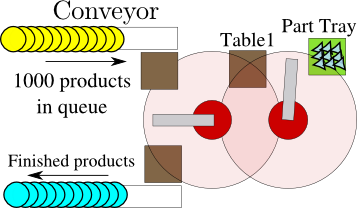
\includegraphics[width=.9\linewidth]{img/model2a.png}

\begin{itemize}
\item factory assembly problem
\begin{itemize}
\item \texttt{cell-assembly}
\end{itemize}
\item gripper + woodworking + logistics.
\begin{itemize}
\item many products -- large scale, repetitive
\item multiple operations -- to complete each product
\item while moving the arms without collision.
\end{itemize}
\item Assembling recipes are provided in the problem
\begin{itemize}
\item while \textbf{optimizing the arm motion}
\end{itemize}
\end{itemize}
\begin{resume}
\begin{itemize}
\item The problem we mainly focus on in this presentation is a factory assembly problem,
\begin{itemize}
\item called cell-assembly. This is a problem inspired by actual factory assembly systems.
\end{itemize}
\item The problem is similar to gripper, plus woodworking, plus logistics.
\begin{itemize}
\item Similar to gripper because there are many products in the conveyor and they are identical.
\item This is also similar to woodworking because multiple operations should be done to complete each product.
\item Finally, this is also similar to logistics because 
the planner should move the robot arms and transport the products.
However it should also avoid collision.
\end{itemize}
\item In this domain, assembling recipes for the products are provided in the problem.
\begin{itemize}
\item Therefore the primary task of a planner is to \textbf{optimize the arm motion}.
\end{itemize}
\end{itemize}
\end{resume}

\subsection{Previous work}
\label{sec-1-1}

\begin{center}
\begin{xlarge}
ACP: Planning with loops,

using the cyclic structure of the domain
\end{xlarge}

\begin{itemize}
\item 6/24 (poster), 6/26 (Session AM 1a: Assembly and Manufacturing) :)
\end{itemize}
\end{center}


\begin{resume}
To solve this kind of problem, I proposed ACP, automated cyclic planner, in my
previous paper. It uses the cyclic structure of the domain.
\begin{itemize}
\item ACP is going to be presented in the poster session tomorrow,
and also in the final day of ICAPS.
\end{itemize}
\end{resume}



\subsection{Previous Work: ACP}
\label{sec-1-2}

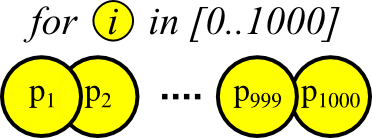
\includegraphics[width=.9\linewidth]{img/indices.png}

\begin{itemize}
\item Provides a framework
\item If all the products are truely indistinguishable
\begin{itemize}
\item i.e. the plan to assemble products are identical
\item except the object index \emph{i}.
\end{itemize}
\end{itemize}

\begin{resume}
\begin{itemize}
\item ACP provided a framework for solving these kind of problem under some restriction.
\item the restriction is, if all the products are truely indistinguishable,
\begin{itemize}
\item in other words the plans of all subproblems,
to assemble the products, are identical
\item except the object index \emph{i}.
\end{itemize}
\item The results of this work in blief is,
\begin{itemize}
\item It manages to construct a loop once and unroll the same plan.
\item and the marginal cost is negligible.
\end{itemize}
\end{itemize}
Today's work is in this line of work.
\end{resume}

\subsection{The Loops in the previous work}
\label{sec-1-3}

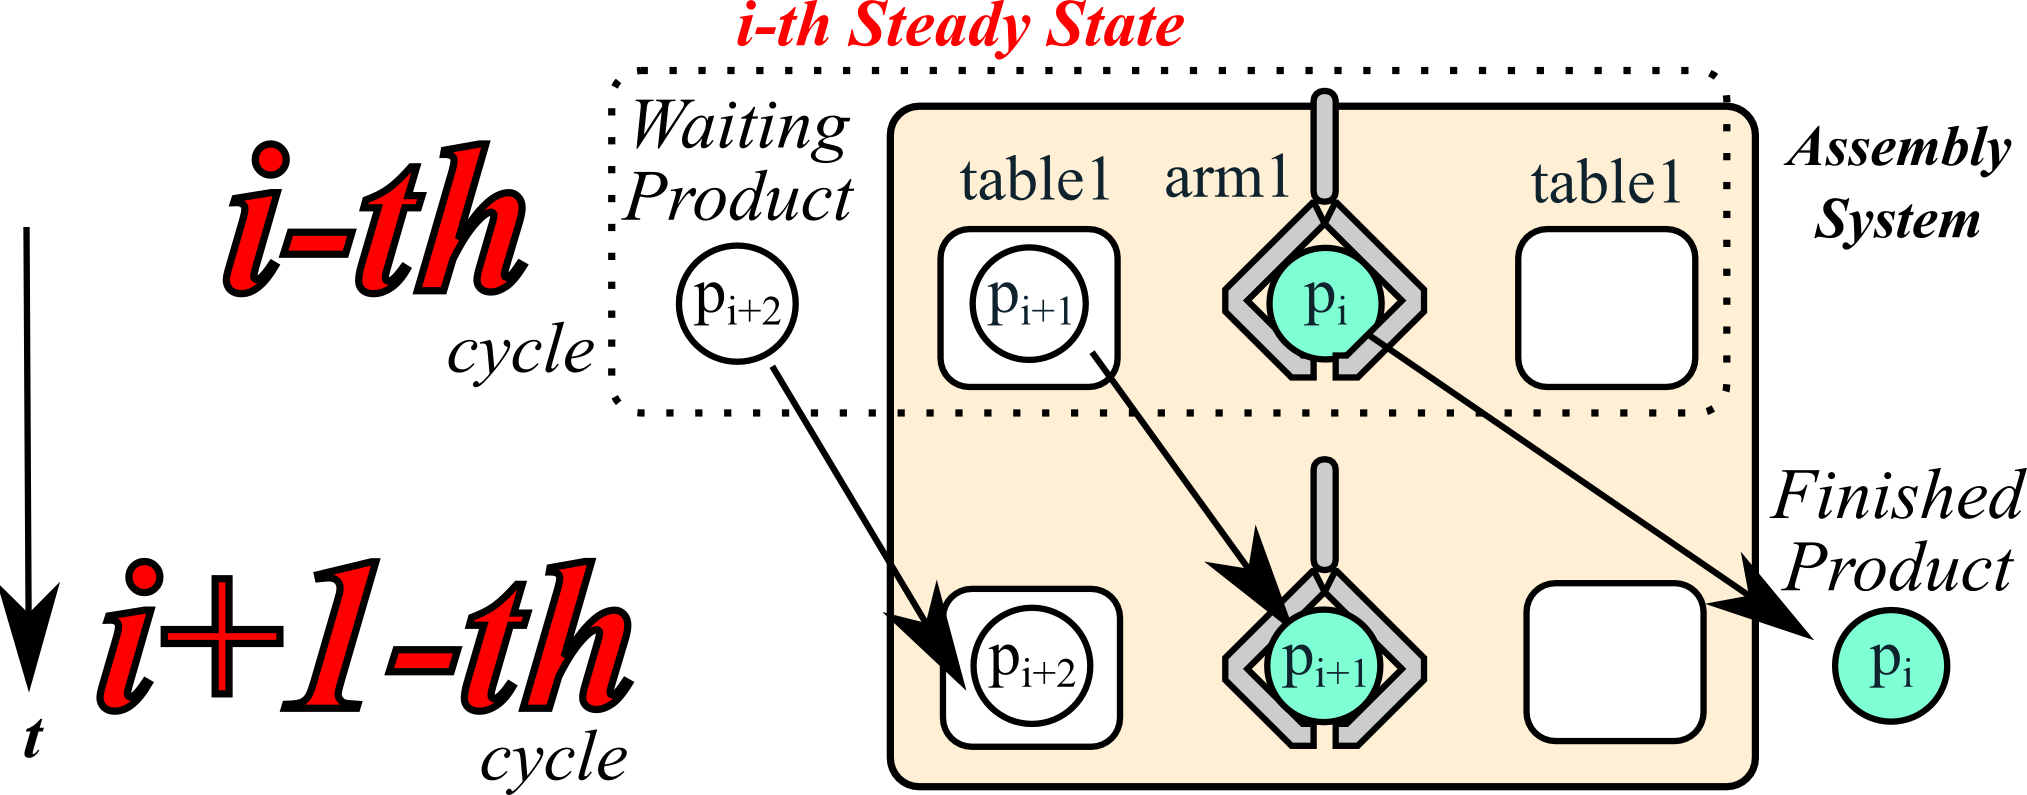
\includegraphics[width=.9\linewidth]{img/steady-state.png}

\begin{resume}
This is the illustration describes the loop structure.
The upper half of the figure describes a state of an assembly system
at some point. We index the state with \emph{i}, and calls it a steady state.
If we update the index \emph{i} to \emph{i+1}, only the indices of objects in a Steady State
changes, but the state of the other objects, such as arms, tables and machines do
not change.
\end{resume}

\subsection{Issues in the previous work}
\label{sec-1-4}

\begin{itemize}
\item 全てのオブジェクトが同じプランで解ける補償はない。
\item オブジェクトがそれ単体で処理できるとは限らない。
\end{itemize}

\subsection{全てのオブジェクトが同じプランで解ける補償はない}
\label{sec-1-5}

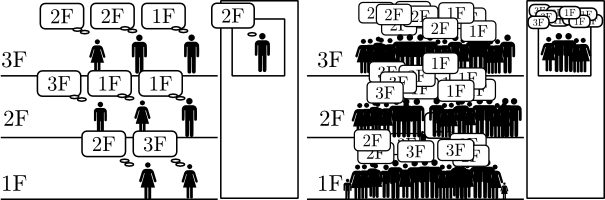
\includegraphics[width=.9\linewidth]{img/elevator.png}

\begin{itemize}
\item それぞれの人は別の初期状態と別のゴール状態を持っている
\item それぞれの部分問題を解くプランは異なる
\end{itemize}


\subsubsection{仕分けすればいい}
\label{sec-1-5-1}

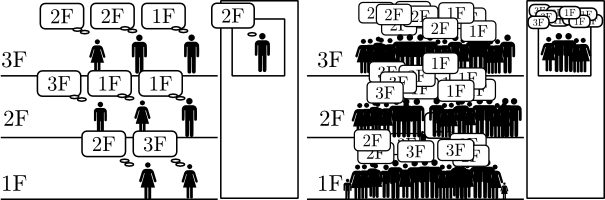
\includegraphics[width=.9\linewidth]{img/elevator.png}

\begin{itemize}
\item 階の数は3つ
\item 1階から2階に行きたい人の数が 一万人 etc\ldots{}
\item 初期条件と終了条件の組は たかだか6個のタイプの製品(=人間)しかない
\item このエレベータ問題だけでなく、一般のIPC問題でも、似たような
繰り返し構造があるのではないか?
\begin{itemize}
\item =見た目ほど難しくないのではないか?
\end{itemize}
\end{itemize}

というのがストーリー

\subsection{オブジェクトがそれ単体で処理できるとは限らない}
\label{sec-1-6}

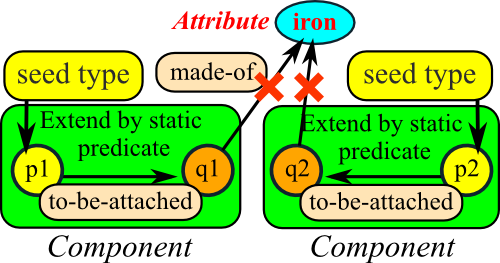
\includegraphics[width=.9\linewidth]{img/abstract-component.png}

たとえ初期状態と終了状態が同じでも、
波線 
\includegraphics[width=.9\linewidth]{img/wave-circle.png} だけをみてループを作ると、 
\includegraphics[width=.9\linewidth]{img/white-circle.png} の番号付けが正
しくなくなってしまう

\emph{やはり仕分けしてしまえば良い。}

\section{large-scale, hetelogeneous repetitive problems}
\label{sec-2}

\begin{itemize}
\item hetelogeneous -- 別々
\item homogeneous -- 同一
\end{itemize}

同一のもののループだけでなく、複数種のループを組み合わせたい。

\subsection{Component Abstraction}
\label{sec-2-1}

\begin{container-fluid}
\begin{row-fluid}
\begin{span6}
\begin{itemize}
\item コンポーネント1
\begin{itemize}
\item 浅井(名前)
\item 浅井の腕
\item 浅井の足
\end{itemize}
\item コンポーネント2
\begin{itemize}
\item 中野(名前)
\item 中野の腕
\item 中野の足
\end{itemize}
\end{itemize}
\end{span6}
\begin{span6}
\begin{itemize}
\item Static Graph を活用して、プランニングのこのような構造を検出する。
\end{itemize}
\end{span6}
\end{row-fluid}
\end{container-fluid}

\subsection{Abstract Type おさらい}
\label{sec-2-2}

\texttt{svg:static-facts}

\subsection{2つ目の課題は解決}
\label{sec-2-3}

これで、

\begin{quote}
たとえ初期状態と終了状態が同じでも、
波線 
\includegraphics[width=.9\linewidth]{img/wave-circle.png} だけをみてループを作ると、 
\includegraphics[width=.9\linewidth]{img/white-circle.png} の番号付けが正
しくなくなってしまう
\end{quote}

の問題が解決

\subsection{Attributes}
\label{sec-2-4}

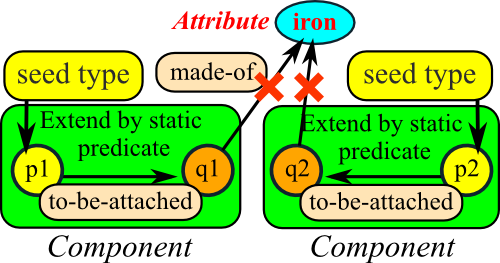
\includegraphics[width=.9\linewidth]{img/abstract-component.png}

\begin{itemize}
\item コンポーネント1
\begin{itemize}
\item 浅井(名前)
\item 浅井の腕
\item 浅井の足
\item アトリビュート : \textbf{髪の毛の色=黒}
\end{itemize}
\item コンポーネント2
\begin{itemize}
\item 中野(名前)
\item 中野の腕
\item 中野の足
\item アトリビュート : \textbf{髪の毛の色=黒}
\end{itemize}
\end{itemize}

\subsection{Abstract Task}
\label{sec-2-5}

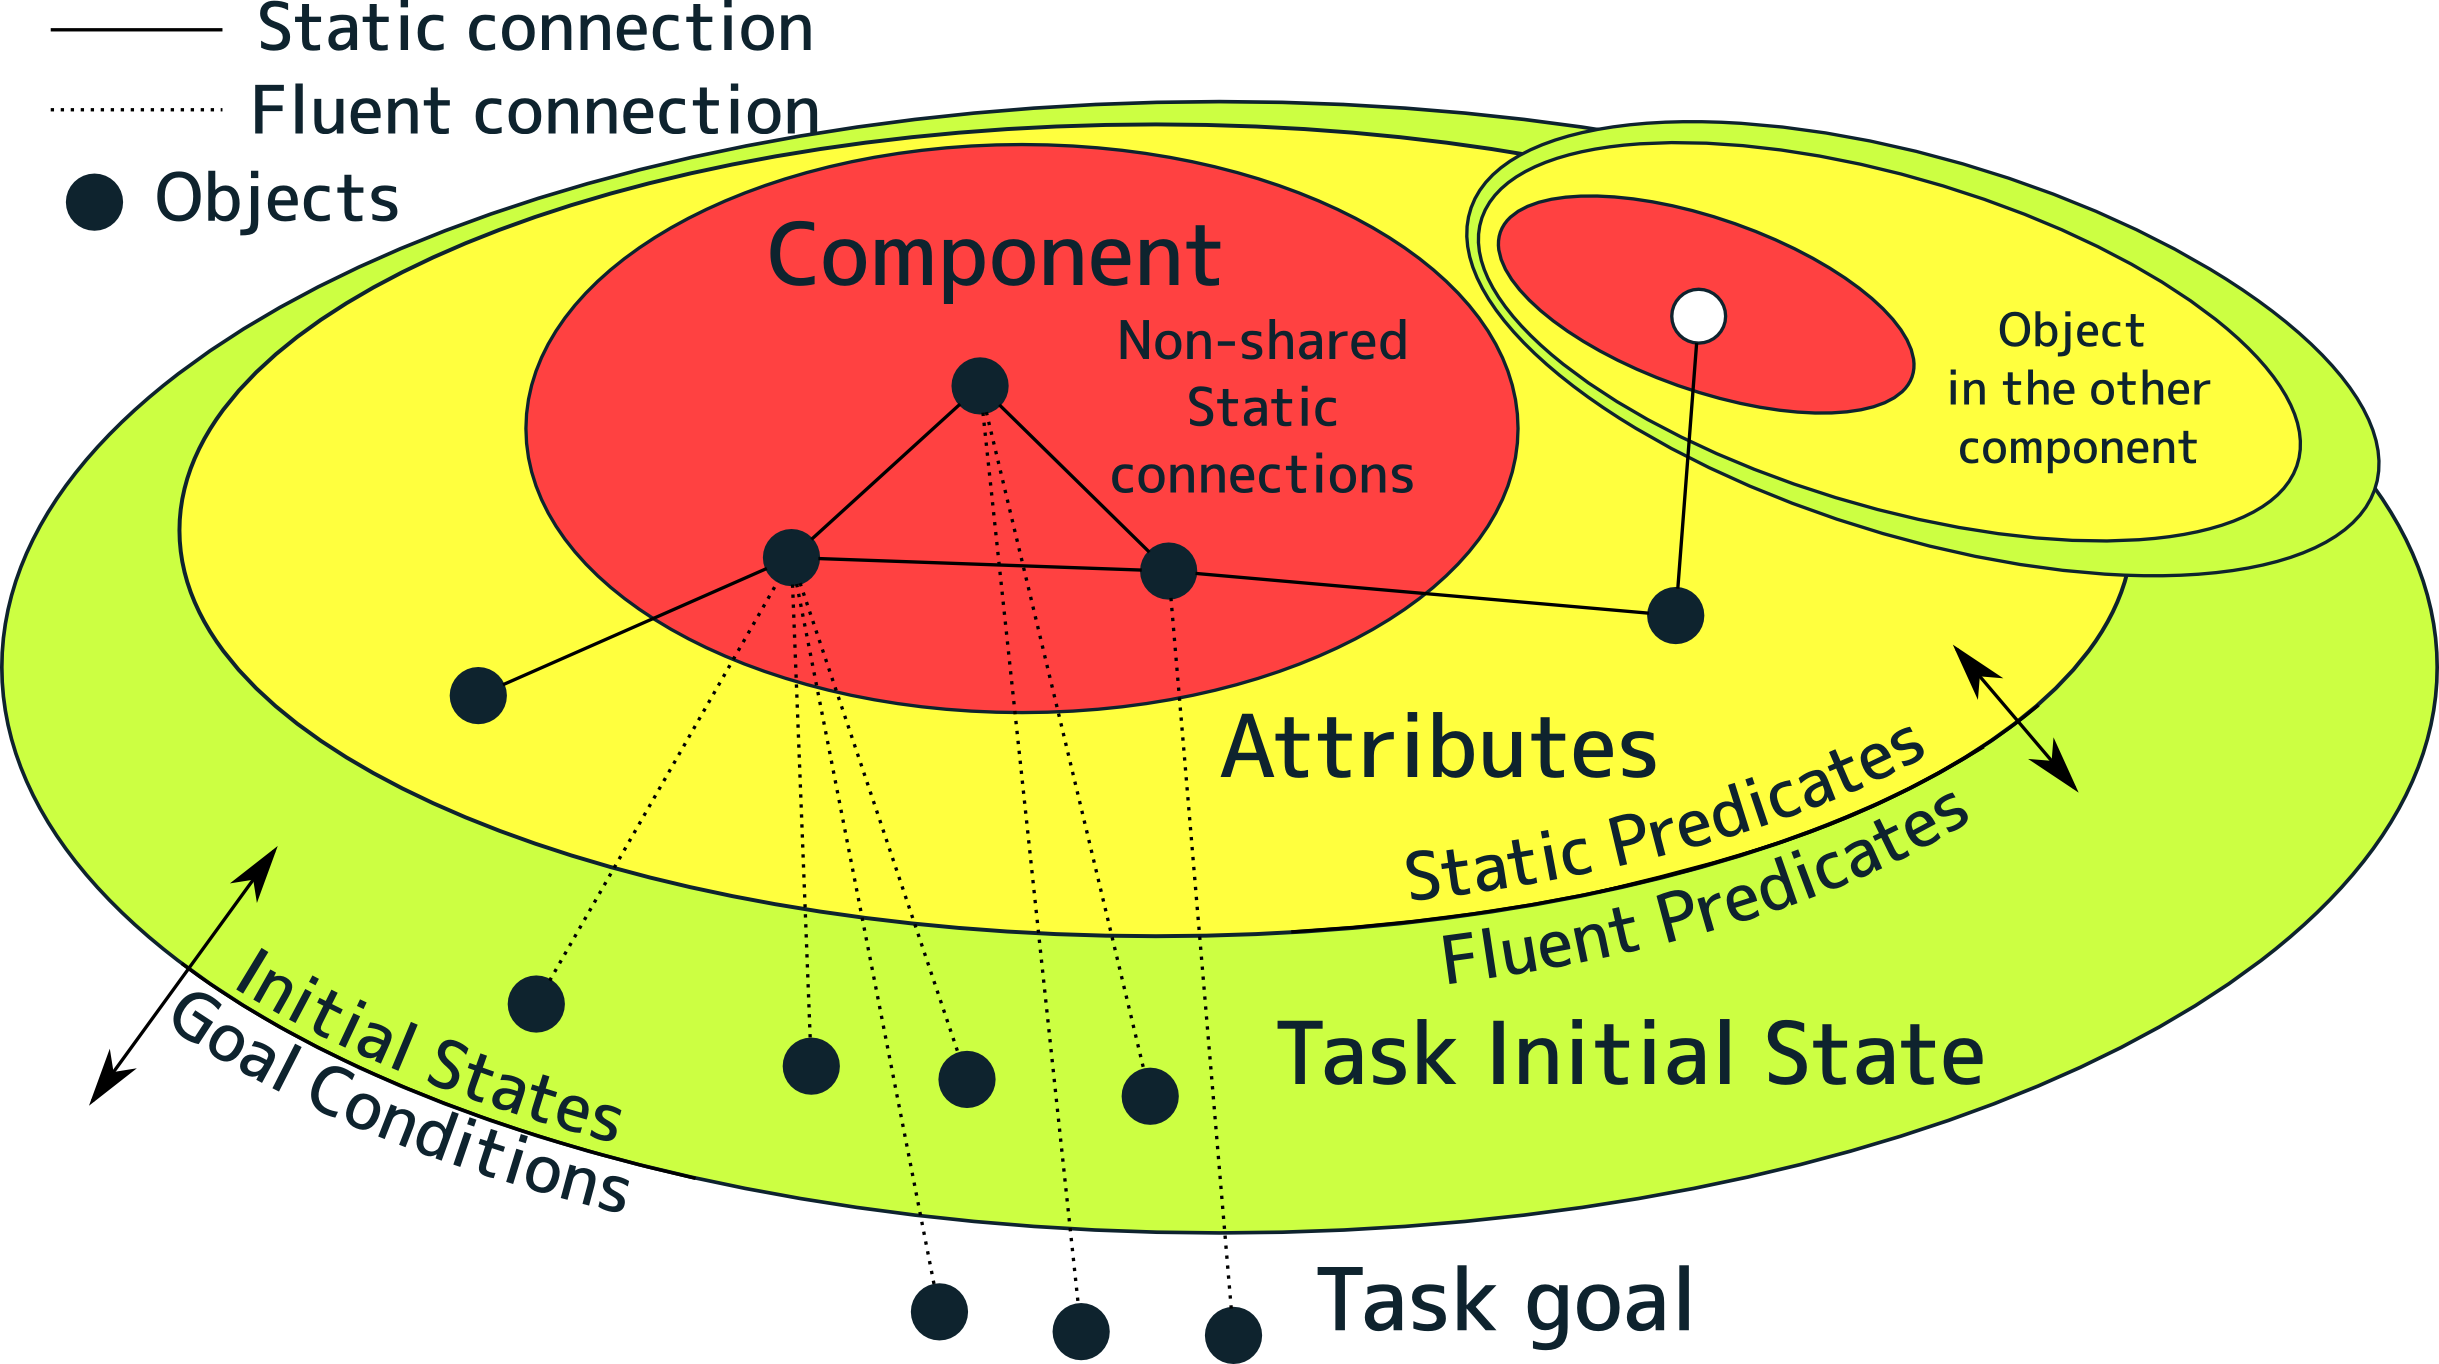
\includegraphics[width=.9\linewidth]{img/abstract-task.png}

\begin{itemize}
\item グループ化されたコンポーネントごとに、初期状態と終了状態を集めてくる
\item --> 1グループだけで問題を解いてみる.
\end{itemize}

\subsection{タスク・プランの互換性}
\label{sec-2-6}

\begin{itemize}
\item 環境オブジェクト + 主題とするコンポーネント \(X\) のみを含む問題を作成
\end{itemize}

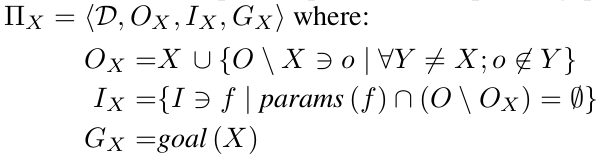
\includegraphics[width=.9\linewidth]{img/static/abstract-task.png}

プランを得て、そのプラン中の X の要素を 別の Y の要素に入れ替え、
プランとして正しかったら \textbf{互換性あり}

\subsection{問題: ときどきUNSAT}
\label{sec-2-7}

オブジェクトを削除したから。

このばあい

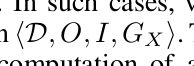
\includegraphics[width=.9\linewidth]{img/static/restoration.png}

Object Restoration を用いる。削除するのをゴールだけにする

\section{結果}
\label{sec-3}

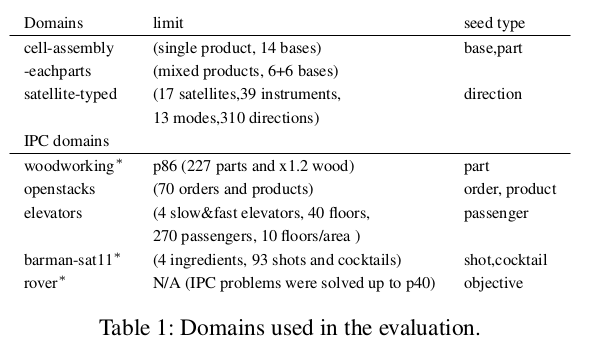
\includegraphics[width=.9\linewidth]{img/static/eval.png}

既存プランナの限界を調べてから、その限界のところで勝負!

\subsection{結果}
\label{sec-3-1}

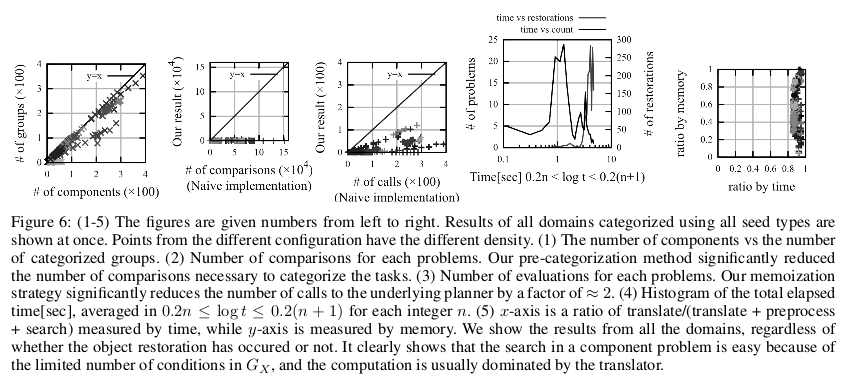
\includegraphics[width=.9\linewidth]{img/static/result.png}
